\PassOptionsToPackage{svgnames}{xcolor}
\documentclass[11pt,a4paper]{article}
\usepackage[utf8]{vietnam}
\usepackage{graphicx}
\usepackage{tikz}
\usepackage[object=vectorian]{pgfornament} %%  http://altermundus.com/pages/tkz/ornament/index.html
\usepackage{lipsum}
\usetikzlibrary{calc}
\usepackage[top=2cm, bottom =2cm, right=2cm, left=2.5cm]{geometry}
\usepackage{algorithm}
\usepackage{algorithmic}
\thispagestyle{empty}
\usepackage{transparent}
\usepackage{eso-pic}
\usepackage{enumitem}
\usepackage{xfrac}
\usepackage{graphicx}
\usepackage{multicol}
\newcommand\BackgroundPic{%
\put(0,0){%
\parbox[b][\paperheight]{\paperwidth}{%
\vfill
\centering
{\transparent{0.2} 
\includegraphics[width=\paperwidth,height=\paperheight,%
keepaspectratio]{Logo_hcmus.png}}%
\vfill
}}}
\newcommand{\sectionline}{%
  \noindent
  \begin{center}
  {\color{DarkViolet}
    \resizebox{0.5\linewidth}{1ex}
    {{%
    {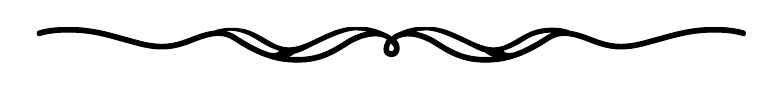
\begin{tikzpicture}
    \node  (C) at (0,0) {};
    \node (D) at (9,0) {};
    \path (C) to [ornament=85] (D);
    \end{tikzpicture}}}}}%
    \end{center}
}
%% A macro with two arguments to change ornaments and colors easily
%% Syntax -- \sectionlinetwo{<color>}{<ornament>}
\newcommand{\sectionlinetwo}[2]{%
  \nointerlineskip \vspace{.5\baselineskip}\hspace{\fill}
  {\color{#1}
    \resizebox{0.8\linewidth}{2ex}
    {{%
    {\begin{tikzpicture}
    \node  (C) at (0,0) {};
    \node (D) at (9,0) {};
    \path (C) to [ornament=#2] (D);
    \end{tikzpicture}}}}}%
    \hspace{\fill}
    \par\nointerlineskip \vspace{.5\baselineskip}
  }
  
\usepackage{tocloft}

\advance\cftsecnumwidth 0.5em\relax
\advance\cftsubsecindent 0.5em\relax
\advance\cftsubsecnumwidth 0.5em\relax
  
\renewcommand{\thesection}{\Roman{section}.} 

\usepackage{hyperref}
\hypersetup{hidelinks}
%\hrefstyle{same}

\begin{document}
\AddToShipoutPicture*{\BackgroundPic}
\ClearShipoutPicture
\begin{tikzpicture}[remember picture,overlay]
  \draw[line width = 1pt] ($(current page.north west) + (0.5in,-0.5in)$) rectangle ($(current page.south east) + (-0.5in,0.5in)$);
  \end{tikzpicture}
 \begin{center}

 \LARGE {\textbf{TRƯỜNG ĐẠI HỌC KHOA HỌC TỰ NHIÊN}} \\
 %\scriptsize{ĐẠI HỌC QUỐC GIA - THÀNH PHỐ HỒ CHÍ MINH} \\
 \large{\textbf{ĐẠI HỌC QUỐC GIA - THÀNH PHỐ HỒ CHÍ MINH}}\\[.2in]
 %\rule{4in}{0.01cm}

\sectionlinetwo{Black}{88}
 \vspace{2in}
 %
\includegraphics[scale=0.2]{Logo_hcmus.png}\\
 
 \Huge{\textbf{REPORT}}\\
 \vspace{.2in}
 \end{center}
 
\center{\textbf{\huge{SORTING ALGORITHMS:}} \vspace{0.1in}\\\Large{\textit{\textbf{IDEA, TIME PERFORMANCE, DATA ANALYSE}}}}
\vspace{1in}

\begin{flushleft}
\large{\textbf{\textit{GROUP MEMBERS:}}}
\end{flushleft}

\begingroup
\setlength{\tabcolsep}{10pt}
\renewcommand{\arraystretch}{1.2}
\LARGE
\begin{flushleft}
\begin{tabular}{l l l}
\textbf{21127403}  & \hspace{.1in} \textbf{Nguyễn Minh Quân}\\
\textbf{21127664}  & \hspace{.1in} \textbf{Trần Đại Niên}\\
\textbf{21127602}  & \hspace{.1in} \textbf{Nguyễn Hoàng Duy}\\
\textbf{21127718}  & \hspace{.1in} \textbf{Lưu Vĩnh Tuấn}\\
\end{tabular}\\
\end{flushleft}
\endgroup

\vspace{0.1in}

\begin{flushleft}
\large{\textbf{\textit{INTRUCTORS:}}}
\end{flushleft}

\begingroup
\setlength{\tabcolsep}{10pt}
\renewcommand{\arraystretch}{1.2}
\LARGE
\begin{center}
\begin{tabular}{l r}
\textbf{Văn Chí Nam} & \hspace{4cm} \textbf{Bùi Huy Thông} \\
\textbf{Lê Thanh Tùng}  & \hspace{4cm} \textbf{Trần Thị Thảo Nhi}\\
\end{tabular}\\
\end{center}
\endgroup
\vspace{.1in}

\sectionlinetwo{Black}{88}

\pagebreak
\captionsenglish{ 
	\tableofcontents
}
\pagebreak
\flushleft{
	\section{Introduction}
	The project is about doing research on some common  and basic sorting algorithms. We will learn about how each algorithm works, 
	how it performs with different order of data(random/ reversed sorted/ nearly sorted/ sorted array), 
	what its application in real life, some advantage and disavantage of each algorithm. With all the knowledge from these algorithm, we will make a application
	for the user to know what is the runtime and how many comparisons a specific algorithm takes to sort the whole array. The user can define the data range, the order of data then the data will 
	be generated automatically or using data from input file. User can ask program to return the output from one algorithm or two algorithm simultaneously.
	\\[12pt]Through this project, we have a oppoturnity to work as a group and practice reading research and take in some new knowledge and understand more
	about how the data is sorted in different ways. And with the support from our teachers, we are able to do the research more efficiently and know what need to be done in order to 
	accomplish our goals. So our group members are extremely thankful to our teacher: Dr. Van Chi Nam, Mr. Bui Huy Thong, Ms. Tran Thi Thao Nhi, Mr. Le Thanh Tung for putting so much 
	effort to help us to achieve our goals.
	\\[12pt]All the code is coded in C\texttt{++}. the report is written in \LaTeX  \hspace{1pt} and all hreferences we used are mentioned in the hreference section at the end of the report.
	\pagebreak
	\section{Algorithm Presentation}
		\subsection{Selection Sort}
			\begin{enumerate}
				\item \textbf{Main idea:}
				
				The selection sort simply partition the list into two main logical parts, the sorted part and the unsorted part. Any iteration picks a value from the unsorted and places it in the sorted list, making the sort partition grow in size while the unsorted partition shrinks for each iteration. When adding to the sorted list, the algorithm makes sure that the value is added at the right position to ensure an order sequence of the sorted partition. The process is terminated when the number of items or the size of the unsorted is one (1). The procedure to select a value to be moved to the sorted list will return minimum value or maximum value in the unsorted partition, which will be swapped to position the item correctly. 
				\\[12pt]
				\item \textbf{Pseudo code:}
				
				
			\end{enumerate}
		
		\subsection{Insertion Sort}
			\begin{enumerate}[label=\textbf{\arabic*})]
				\item \textbf{Main idea:}
			
				It works similar to the way you sort playing cards in your hands. The array is virtually split into a sorted and an unsorted part. Values from the unsorted part are picked and placed at the correct position in the sorted part.
				\\[12pt]
				\item \textbf{Pseudo code:}
				
				\begin{algorithm}
					\caption{Insertion Sort}
					\begin{algorithmic} 
						\STATE $i \leftarrow 1$
						\WHILE {$i < length(A)$}
						\STATE $x \leftarrow A[i]$
						\STATE $j \leftarrow i - 1$ 
						\WHILE {$j \ge 0$ \AND $A[j] > x$}
						\STATE $A[j+1] \leftarrow A[j]$
						\STATE $j \leftarrow i - 1$ 
						\ENDWHILE
						\STATE $A[j+1] \leftarrow x$ 
						\STATE $i \leftarrow i + 1$ 
						\ENDWHILE
					\end{algorithmic}
				\end{algorithm}
				
				\item \textbf{Flowchart:}
					\begin{figure}[h!]
						\centering
						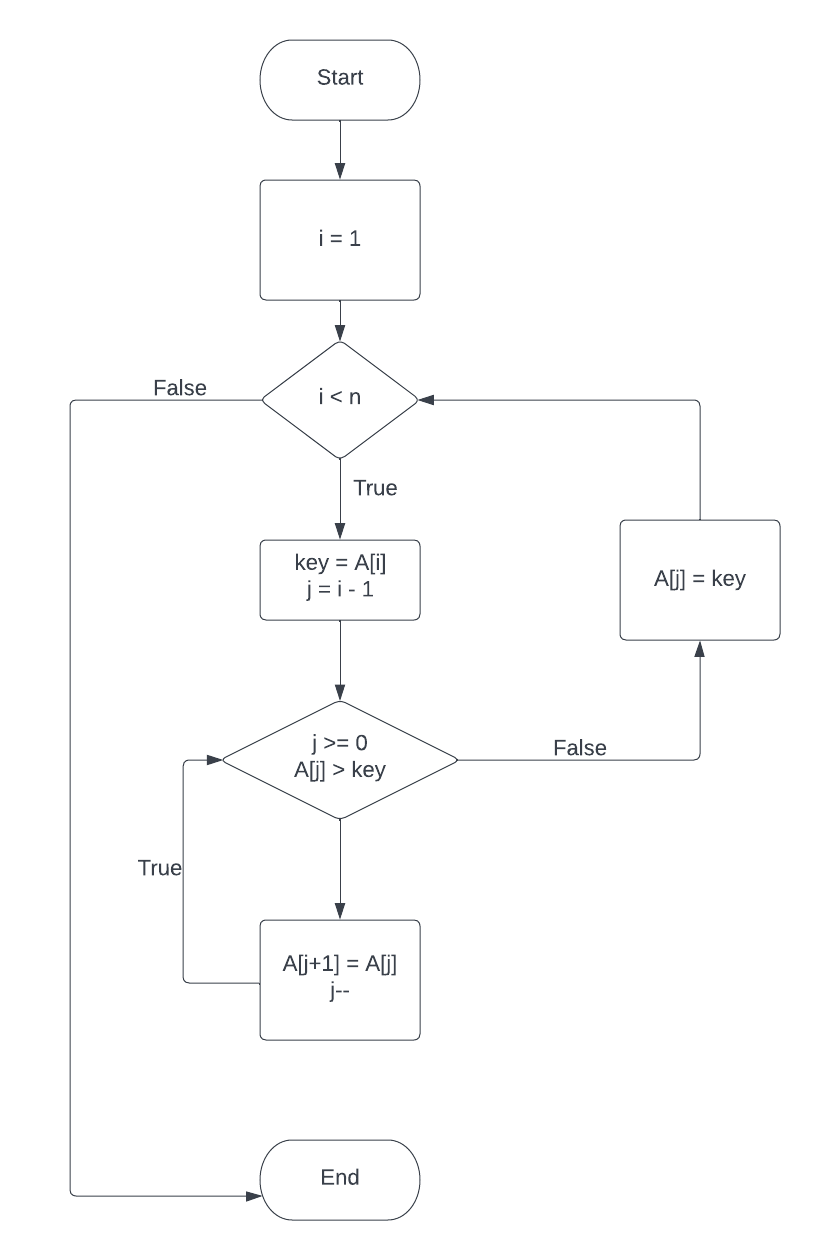
\includegraphics[width=0.5\textwidth]{Insertion Sort}
					\end{figure}
					
				\item \textbf{Description:}
					To sort an array of size N in ascending order: 
						\begin{itemize}
							\item Iterate from A[1] to A[N] over the array. 
							\item Compare the current element (x) to its predecessor. 
							\item If the key element is smaller than its predecessor, compare it to the elements before. Move the greater elements one position up to make space for the swapped element.
						\end{itemize}
				\item \textbf{Variants/ improvements:}
					\begin{itemize}
						\item Shell sort compares elements separated by a distance that decreases on each pass. Shell sort has distinctly improved running times in practical work, with two simple variants requiring $\mathcal{O}(n^{\sfrac{3}{2}})$ and $\mathcal{O}(n^{\sfrac{4}{3}})$ running time
						\item Binary insertion sort employs a binary search to determine the correct location to insert new elements, and therefore performs $\lceil log_{2}n \rceil$ comparisons in the worst case. When each element in the array is searched for and inserted this is $\mathcal{O}$(n log n). The algorithm as a whole still has a running time of $\mathcal{O}(n^2)$ on average because of the series of swaps required for each insertion
						that this sorting algorithm runs with high probability in $\mathcal{O}$(n log n) time.
						\item binary merge sort uses a binary insertion sort to sort groups of 32 elements, followed by a final sort using merge sort. It combines the speed of insertion sort on small data sets with the speed of merge sort on large data sets.
						\item library sort or gapped insertion sort that leaves a small number of unused spaces (i.e., "gaps") spread throughout the array. The benefit is that insertions need only shift elements over until a gap is reached. The authors show that this sorting algorithm runs with high probability in $\mathcal{O}$(n log n) time.
					\end{itemize}
				\item \textbf{Advantage, disadvantage:}
					\begin{table}[ht]
						\centering
						\begin{tabular}{|p{8cm}|p{8cm}|}
							\hline
							\textbf{Advantage} & \textbf{Disadvantage} \\
							\hline
							\hline
							The main advantage of the insertion sort is its simplicity. 							 & The disadvantage of the insertion sort is that it does not perform as well as other, better sorting algorithms \\[12pt]
							It also exhibits a good performance when dealing with a small list. 					 & With n-squared steps required for every n element to be sorted, the insertion sort does not deal well with a huge list. \\[12pt]
							The insertion sort is an in-place sorting algorithm so the space requirement is minimal. & The insertion sort is particularly useful only when sorting a list of few items. \\
							\hline
						\end{tabular}
					\end{table}
				\item \textbf{Application:}	
					\begin{itemize}
						\item If the cost of comparisons exceeds the cost of swaps, as is the case for example with string keys stored by reference or with human interaction, then using binary insertion sort may yield better performance.
						\item A variant named binary merge sort uses a binary insertion sort to sort groups of 32 elements, followed by a final sort using merge sort.
						\item If a skip list is used, the insertion time is brought down to $\mathcal{O}$(log n), and swaps are not needed because the skip list is implemented on a linked list structure. The final running time for insertion would be $\mathcal{O}$(n log n).
					\end{itemize}
			\end{enumerate}
			
		\subsection{Bubble Sort}
		\subsection{Shaker Sort}
		\subsection{Shell Sort}
		\subsection{Heap Sort}
		\subsection{Merge Sort}
		\subsection{Quick Sort}
		\subsection{Counting Sort}
		\subsection{Radix Sort}
		\subsection{Flash Sort}
	\section{Experimental results and comments}
	\section{Project organization and Programming notes}
	
	% Counting sort:
	
	% \\[12pt]
	
	% Radix sort:
	
	% \\[12pt]
	
	% Flash sort:
	% \href{https://en.wikipedia.org/wiki/Flashsort}
	
	\begin{thebibliography}{}
		\bibitem{} \href{https://www.codeproject.com/Questions/164306/convert-argv-to-something-and-back}{Convert argv to something and back}
		\bibitem{} \href{https://techvidvan.com/tutorials/selection-sort/}{Selection Sort}
		\bibitem{} \href {http://csir.org.gh/images/Doc/Refereed_Journal_Articles/Improved%20Selection%20Sort%20Algorithm.pdf}{Improved Selection Sort Document}
		\bibitem{} \href{https://www.liquisearch.com/selection_sort/variants}{Selection Sort Variants}
		\bibitem{} \href{https://dbmspoly.blogspot.com/p/advantage-disadvantages-of-sort.html}{Selection Sort Advantage disadvantage}
		\bibitem{} \href{https://en.wikipedia.org/wiki/Bubble_sort}{Bubble Sort Idea}
		\bibitem{} \href{https://www.geeksforgeeks.org/bubble-sort/}{Bubble Sort Source Code}
		\bibitem{} \href{http://dbmspoly.blogspot.com/p/advantage-disadvantages-of-sort.html}{Bubble Sort Advantage Disadvantage}
		\bibitem{} \href{https://www.geeksforgeeks.org/cocktail-sort/}{Cocktail Sort}
		\bibitem{} \href{https://en.wikipedia.org/wiki/Cocktail_shaker_sort}{Cocktail Shaker Sort}
		\bibitem{} \href{https://en.wikipedia.org/wiki/Shellsort}{Shell Sort Idea}
		\bibitem{} \href{https://www.geeksforgeeks.org/shellsort/}{Shell Sort Source Code}
		\bibitem{} \href{https://www.tutorialspoint.com/Heap-Sort}{Heap Sort}
		\bibitem{} \href{https://techvidvan.com/tutorials/heap-sort/}{Heap Sort}
		\bibitem{} \href{https://www.liquisearch.com/heapsort/variations}{Heap Sort Variants}
		\bibitem{} \href{https://www.quora.com/What-are-the-benefits-of-heap-sort-and-its-disadvantages-compared-to-other-sorting-algorithms}{Advantage and Disadvantage of Heap Sort}
		\bibitem{} \href{https://www.interviewkickstart.com/learn/heap-sort#:~:text=Applications%20of%20Heap%20Sort,-Implementation%20of%20priority&text=Because%20algorithms%20like%20merge%20sort,an%20almost%20sorted%20array%2C%20etc.}{Heap Sort Document}
		\bibitem{} \href{https://www.geeksforgeeks.org/merge-sort/}{Merge Sort}
		\bibitem{} \href{http://dbmspoly.blogspot.com/p/advantage-disadvantages-of-sort.html}{Advantage and Disadvantage of Merge Sort}
		\bibitem{} \href{https://en.wikipedia.org/wiki/Quicksort}{Quick Sort}
		\bibitem{} \href{https://www.geeksforgeeks.org/quick-sort/}{Quick Sort Source Code}
		\bibitem{} \href{https://www.geeksforgeeks.org/counting-sort/}{Counting Sort Source Code}
		\bibitem{} \href{https://www.simplilearn.com/tutorials/data-structure-tutorial/counting-sort-algorithm#:~:text=Applications%20of%20Counting%20Sort%20Algorithm&text=It%20has%20an%20O(n,using%20partial%20hashing%20(1).}{Counting Sort Idea}
		\bibitem{} \href{https://www.interviewkickstart.com/learn/counting-sort}{Counting Sort}
		\bibitem{} \href{https://www.geeksforgeeks.org/radix-sort/}{Radix Sort Source Code}
		\bibitem{} \href{https://www.programiz.com/dsa/radix-sort}{Radix Sort Idea}
		\bibitem{} \href{https://www.interviewkickstart.com/learn/radix-sort-algorithm}{Radix Sort Advantage and Disadvantage}
		\bibitem{} \href{https://en.wikipedia.org/wiki/Flashsort}{Flash Sort Idea}
	\end{thebibliography}
}	

\end{document}

%ve het hinh roi cho nhan xet tong the
